\subsection{Неравенство зон}\label{subsec:inequality}
Когда я заметил, что зоны, на которые Adobe Illustrator делит изображение, могут очень сильно отличаться в размере (отношение площадей может достигать 1000 раз),
мне захотелось измерить это неравенство численно, чтобы при разработке нового алгоритма измерять его качество в том числе по этому параметру.

Существует большое количество метрик, я решил выбрать основные из них:
\begin{itemize}
    \item Индекс Джини (вместе с кумулятивным графиком распределения дохода (также известен как \href{https://en.wikipedia.org/wiki/Lorenz_curve}{кривая Лоренца}))
    \item Процент «дохода» 1\% самых богатых от общего «дохода» (В случае зон вместо дохода используется занимаемая площадь).
    \item Процент самых богатых, имеющих в сумме 50\% от общего дохода.
\end{itemize}

Индекс Джини рассчитывается как отношение площади между кривой Лоренца и «линией равенства» к площади под линией равенства.
Иными словами, $G = \frac{A}{A + B}$ на этой схеме:

\begin{figure}[h!]\label{fig:lorenz_curve}
    \centering
    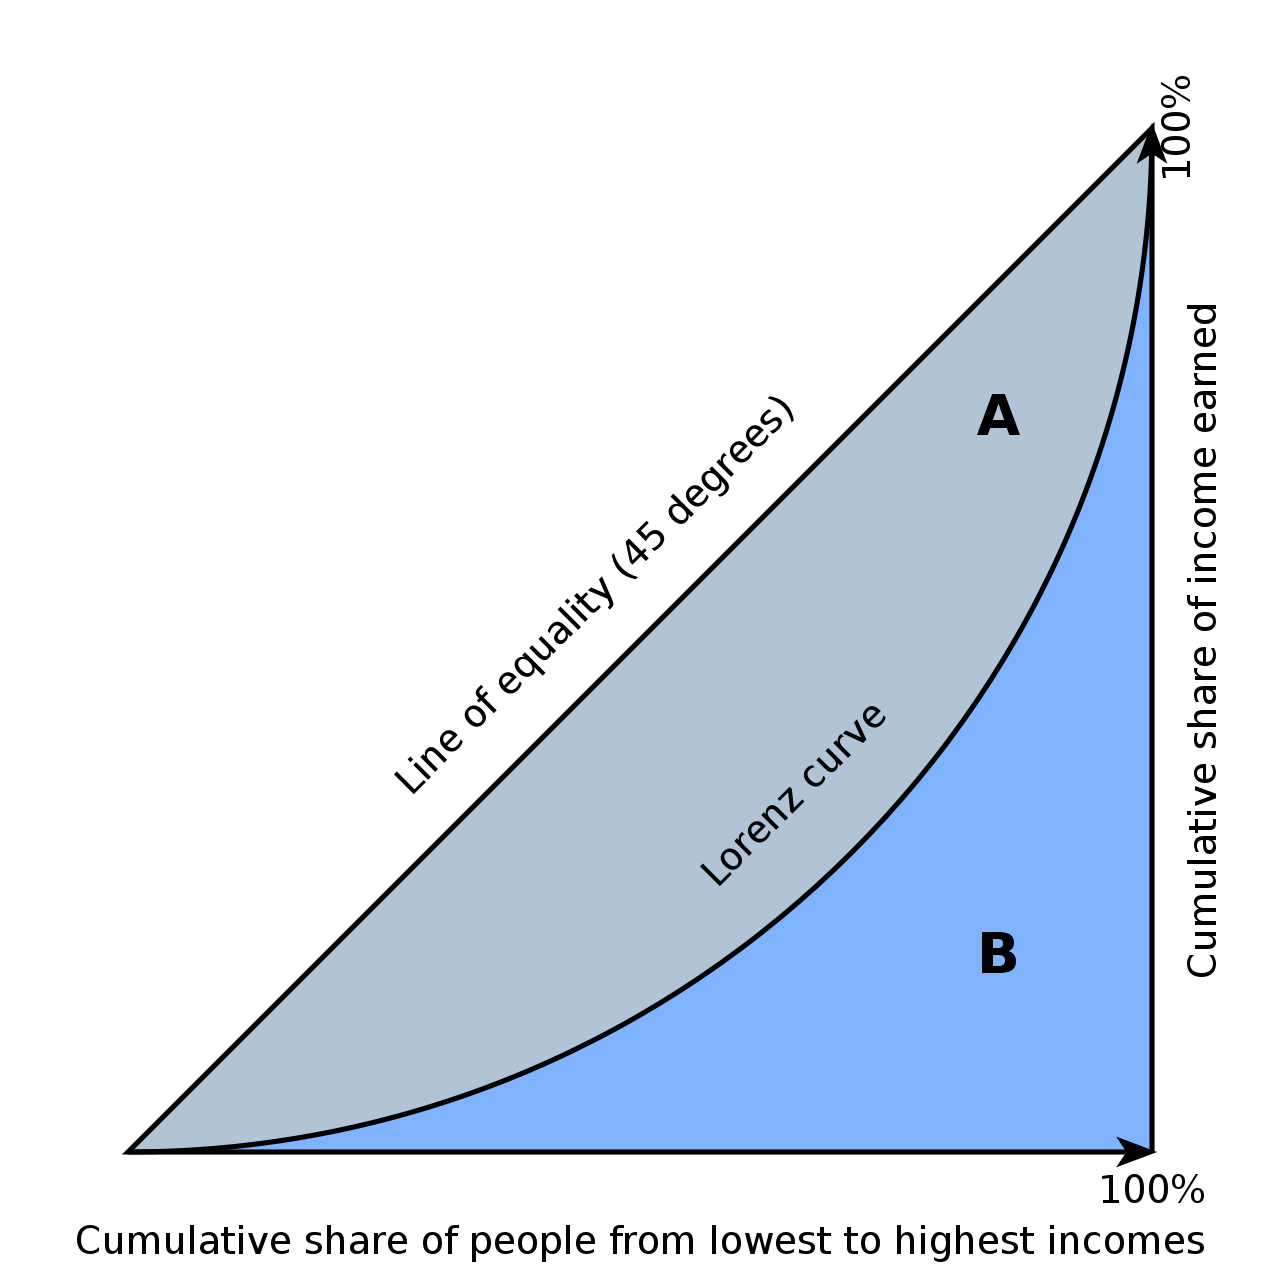
\includegraphics[width=0.75\textwidth]{typical_lorenz_curve.png}
    \caption{Типичная кривая Лоренца}
\end{figure}
Альтернативный способ посчитать коэффициент, использующийся в реализации:
\begin{equation}
    G = \frac{\sum_{i=1}^{n}  \sum_{j=i+1}^{n}  \left| y_i - y_j \right|}{n \cdot \sum_{i=1}^{n} y_i}
\end{equation}
Чем индекс выше, тем большее неравенство наблюдается в стране.
Более того, использование именно этой метрики позволяет комплексно оценить неравенство между анализируемыми объектами —
в отличие от рассмотрения процентов дохода заданного квантиля.


Результаты оказались впечатляющими:
\begin{itemize}
    \item $Gini\_index \approx 76\%$
    \item 1\% крупнейших зон покрывают ≈ 18\% изображения
    \item 6.25\% зон покрывают половину изображения
\end{itemize}

Так выглядит кумулятивный график распределения площади:
\begin{figure}[h!]\label{fig:cumulative_inequality_graph}
    \centering
    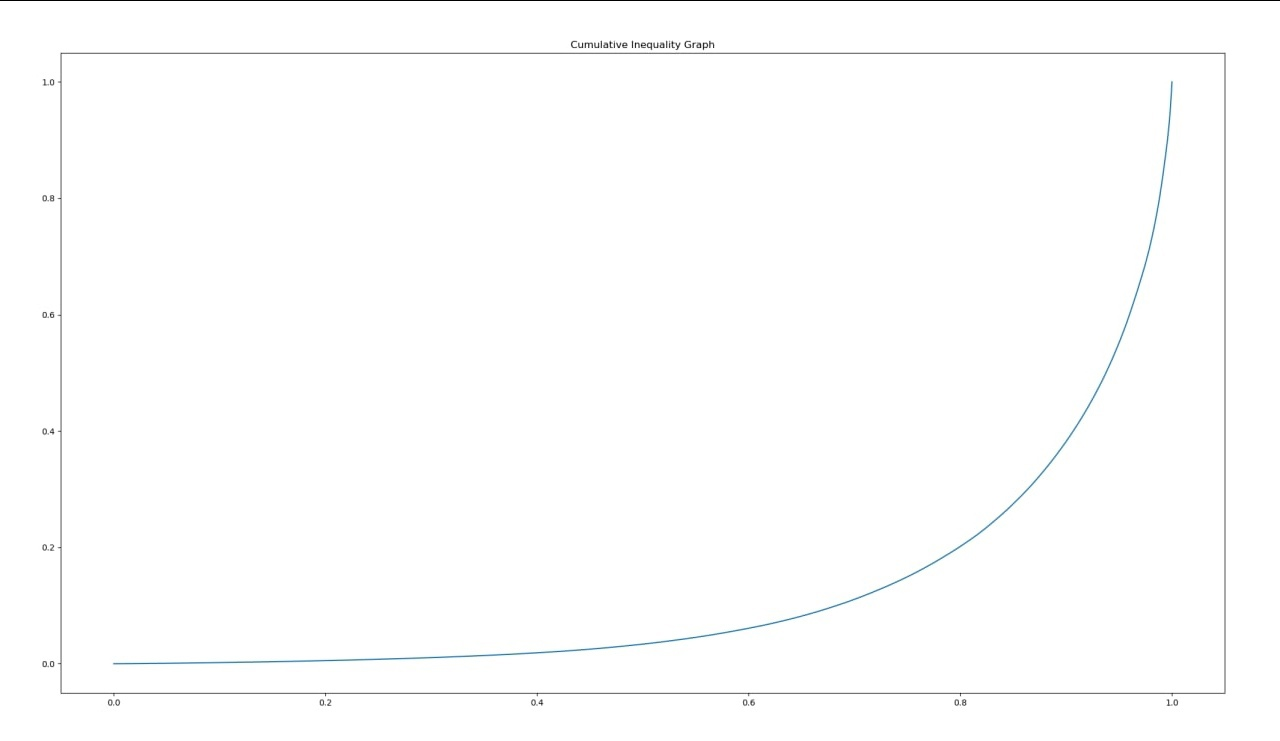
\includegraphics[width=0.75\textwidth]{cumulative_inequality_graph.jpg}
    \caption{Кривая лоренца для зон}
\end{figure}

Нетрудно заметить, что ни в одной стране мира нет такого неравенства, как среди зон:

\begin{figure}[h!]\label{fig:gini_index_world}
    \centering
    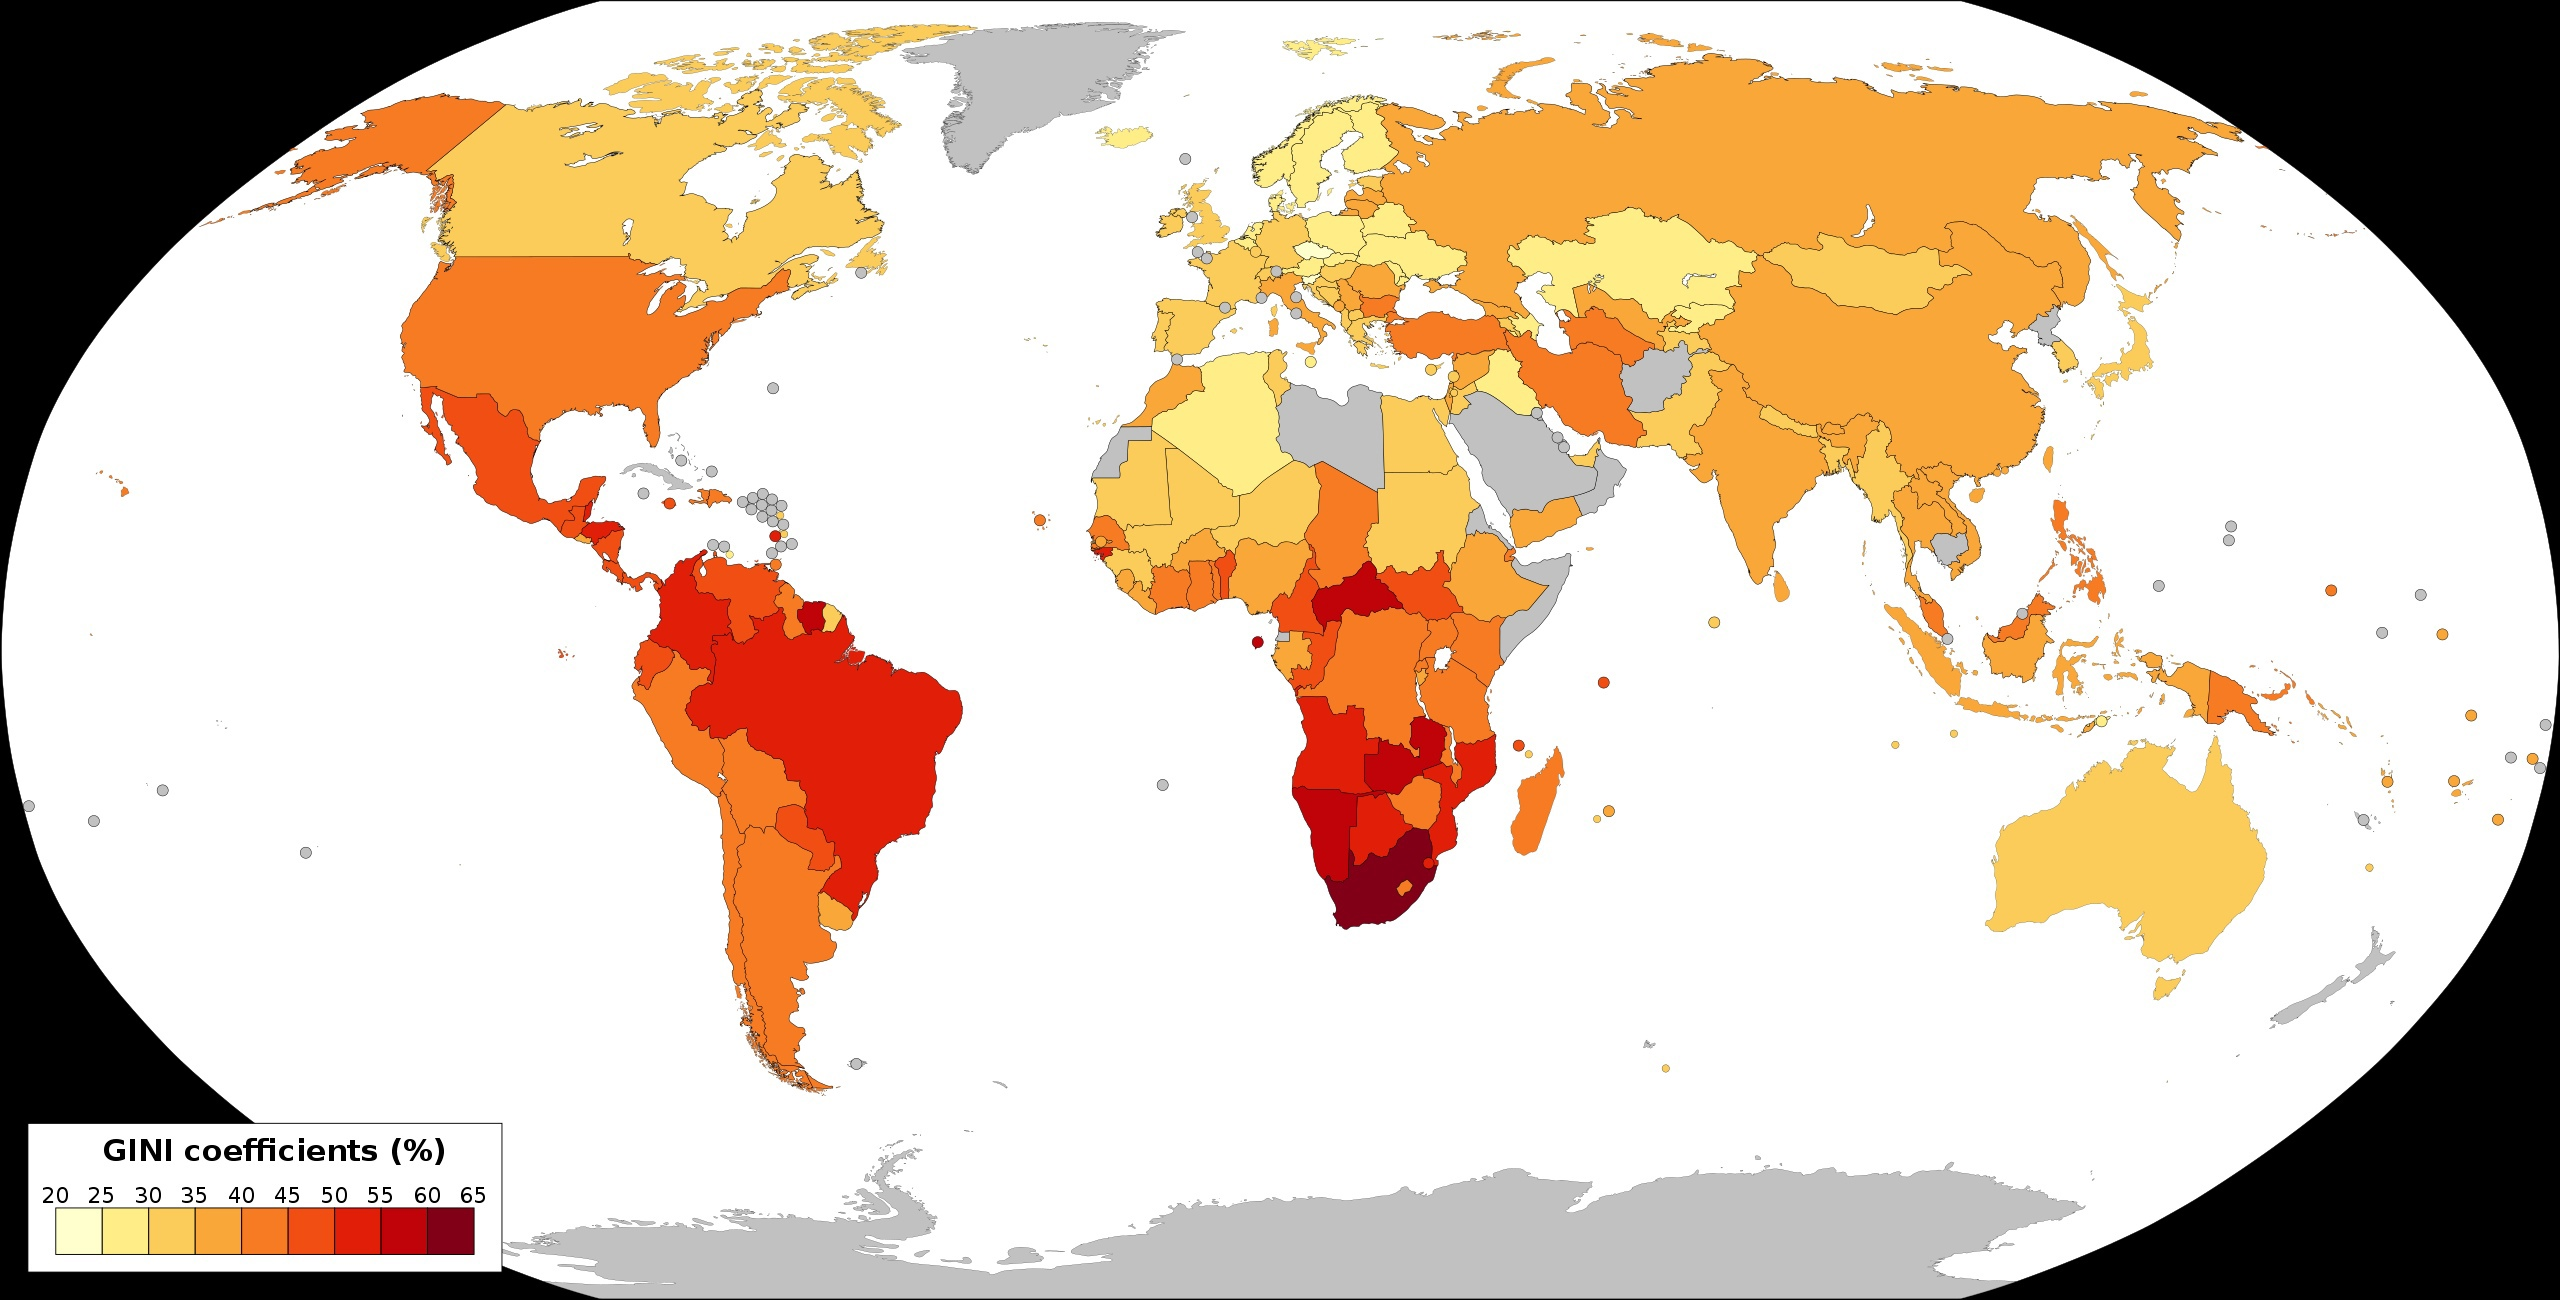
\includegraphics[width=0.75\textwidth]{gini_index_world.jpg}
    \caption{Индекс Джини по странам мира}
\end{figure}
Даже в ЮАР индекс Джини составляет 57.8\%.